\documentclass[a4paper,9pt,russian]{article}
\usepackage{cmap}
\usepackage{hyperref}
\usepackage[T2A]{fontenc}
\usepackage[utf8]{inputenc}
\usepackage[russian]{babel}
\usepackage{graphicx}
\usepackage{xcolor}
\usepackage{amssymb}
\usepackage{amsmath}
\usepackage{physics}

\definecolor{block-gray}{gray}{0.90}
\definecolor{pink}{cmyk}{0,1,0.25,0}

\title{Конспект лекции по теме: ''Обыкновенные дифференциальные уравнения''}
\author{А. В. Козлов}

\begin{document}
\maketitle
\begin{abstract}
    В лекции от 10 апреля 2020 года рассмотрены различные численные методы решения обыкновенных дифференциальных уравнений и их систем. 
    \par Преподаватель: {\sc Алексей Антониевич Балакин}.
\end{abstract}
\tableofcontents
\newpage
\section{Введение}
     Данная лекция посвящена численным методам решения систем обыкновенных дифференциальных уравнений.
\section{Задача Коши}
    Задачей Коши называют задачу на нахождение решения обыкновенного дифференциального уравнения при задании всех значений переменных в некоторой точке, называемой {\it начальной точкой}.
\subsection{Обыкновенные дифференциальные уравнения (ODE)}
    {\it Обыкновенное дифференциальное уравнение}~---~это уравнения вида: \\
        \begin{equation}\label{def}
            u^{(p)} = f(x, u, u',\dots, u^{(p-1)}) \quad\quad\quad
            p \in \mathbb{N},
        \end{equation}
    то есть в левой части стоит производная $p$--ого порядка от искомой функции, а справа~---~некоторая функция, зависящая от $x$, от искомой функции $u$ и от первых $(p-1)$ производных.\par
    Такая форма записи (\ref{def}) неудобна~---~брать высокого порядка производную численно сложно и точность плохая. Поэтому вводят формальную замену переменных:
    \begin{equation}\label{2}
        \begin{cases}
            u_k' &=\ u_{k+1} \quad\ k = 0, \ldots, p-1\\
            u_{p-1}'& =\ f(x,u_0,\ldots, u_{p-1})
        \end{cases},
    \end{equation}
    то есть все производные обозначаются за новые независимые переменные. Одно уравнение сводится к системе $p$ обыкновенных дифференциальных уравнений первого порядка. Размерность повышается, но решать становится легче.\par
    Такие уравнения называются {\it обыкновенными} потому, что искомая функция зависит лишь от одной переменной~---~$x$. Уравнения на функции нескольких переменных, содержащие частные производные, так и называют {\it уравнения в частных производных}.\par
    Можно записать систему (\ref{2}) в более компактном виде, используя вектора: $${\bf u}' = {\bf f}(x, {\bf u}).$$\par
    Будем рассматривать {\it задачу Кошу}. Пускай, условия заданы такие: ${\bf u}(x_0)={\bf u_0}$, то есть в какой-то точке $x_0$ заданы значения функции и её первых $(p-1)$ производных. Иногда их задают не явно, а через уравнения, тогда нужно решать систему уравнений в начальной точке.\par
    Из курса дифференциальных уравнений должно быть известно, что решение системы обыкновенных дифференциальных уравнений единственно в некоторой области $D$ тогда и только тогда, когда функция ${\bf f}$ удовлетворяет {\it условию Липшица} в области $D$:
    \begin{equation}\label{liv}
        \exists\ L\ :\ \bigl\|{\bf f}(x, {\bf u_1}) - {\bf f}(x, {\bf u_2})\bigr\| \  \le \ L\bigl\|{\bf u_1}-{\bf u_2}\bigr\|.
    \end{equation}
    То есть найдётся такая постоянная $L$, что удовлетворится неравенство (\ref{liv}).
    \par
    Ещё один подводный камень, который в дальнейшем не будет обсуждаться,~---~{\it хорошая обусловленность задачи}, то есть решение должно быть равномерно устойчивым по Ляпунову. Это означает, что решения, сблизившись однажды, не должны удаляться.
\subsection{Метод ломанных (Эйлера)}
    Самое простое, что можем сделать~---~это взять какую-то сетку $\bigl\{x_n\bigl\}_{n=1}^N$ с малым шагом (вообще говоря, шаг может не быть постоянным, но обычно выбирают равномерную сетку, чтобы не мучиться со сложным видом производных) и разложить искомую функцию ${\bf u}$ в узлах этой сетки в ряд Тейлора: 
\begin{equation}\label{Teylor}
\begin{split}
 {\bf u_{n+1}} & \approx {\bf u_{n}} + h_n{\bf u_{n}'}     +
    \frac{{h_n}^2}{2}{\bf u_{n}''} = \\
    & = {\bf u_{n}} + h_n{\bf f _{n}} + 
    \frac{{h_n}^2}{2}( \partial_x \boldsymbol{f} + (\boldsymbol{f}, \partial_{\bf u}\boldsymbol{f}) ),
\end{split}    
\end{equation}   
	где $h_n$ есть шаг. Ограничиваясь производной первого порядка, получаем {\itсхему Эйлера} для вычисления значения функции в следующей точки сетки по значению в предыдущей:
    \begin{equation}\label{Eyler}
       {\bf u_{n+1}} = {\bf u_{n}} + h_n\ {\bf f}(x_n,\ {\bf u_{n}}).
    \end{equation}\par
    Казалось бы получили хорошую схему, легко реализуемую на ЭВМ. Но она жутко неустойчивая.\par
    Для примера оценим ошибку $z_n = \abs{u_n - u_*(x_n)}$ между нашим решением $u_n$ и точным решением $u_*(x_n)$ в одномерном случае. Получаем оценку:
    \begin{equation}\label{6}
        z_{n+1} = z_n + h_n\ f_u'\ z_n - \frac{{h_n}^2}{2}\ u_n''.
    \end{equation}
    Видно, что из-за второго порядка по шагу ошибка будет нарастать, и делать это она будет достаточно быстро.\par Таким образом 
    {метод Эйлера~---~плохой вариант}.
\subsection{Метод Рунге--Кутта (Runge--Kutta)}
\subsubsection{Метод Рунге--Кутта 2--ого порядка}
    Мы убедились, что в (\ref{Teylor}) учёта только первой производной не достаточно для получения хорошего численного метода решения систем ОДУ. Учтём же теперь вторую производную в разложении (\ref{Teylor}). По теореме Лагранжа \cite{wiki_l} из математического анализа имеем:
    \begin{equation}\label{7}
        {\bf u_{n}''} = \frac{{\bf f}(\tilde x, \tilde {\bf u}) - {\bf f}( x, {\bf u})}{h_n},
    \end{equation}
    где $\tilde x \in[ x_n,\ x_{n-1}]$. Подставляем (\ref{7}) в (\ref{Teylor}):
    \begin{equation*}
     {\bf u_{n+1}} \approx {\bf u_{n}} + h_n{\bf f_n}     +
    \frac{h_n}{2}\qty({\bf f}(\tilde x, \tilde {\bf u}) - {\bf f}( x, {\bf u})).
    \end{equation*}  
    Представляем разность ${\bf f}(\tilde x, \tilde {\bf u}) - {\bf f}( x, {\bf u})$ как разность $\vb{f}_n$ и $\vb{f}_n\qty(x_n + \Delta x,\ \vb u_n + \Delta \vb u)$ с некоторыми постоянными весами. Вводим константы $\alpha, \beta, \gamma$ и $\boldsymbol{\delta}$ так, как показано ниже:    
    \begin{equation}\label{*}
        {\bf u_{n+1}} \approx {\bf u_{n}} + \alpha h_n {\bf f_{n}} + \beta {h_n} {\bf f_{n}}(x_n+\gamma h_n,\ {\bf u_{n}} + \boldsymbol{\delta} h_n).
    \end{equation}
    Разлагаем (\ref{*}) в ряд Тейлора, получаем (\ref{**}). 
    \begin{equation}\label{**}
        {\bf u_{n+1}} \approx {\bf u_{n}} + (\alpha + \beta) h_n {\bf f_{n}} + \beta h_n^2 \bigl\{ \gamma \partial_x {\bf f_n} + (\boldsymbol{\delta},\ \partial_{\bf u}) {\bf f_n} \bigr\}
    \end{equation}
    Последнее равенство сопоставляем с (\ref{Teylor}), откуда находим уравнения на коэффициенты:
    \[
        \alpha + \beta = 1,\quad \beta \gamma = \frac12,\quad \beta \boldsymbol{\delta} = \frac{\bf f_n}2
    \]
    Есть три уравнения на 4 неизвестных коэффициента. Решить эту систему однозначно не возможно, но можно подбирать какие-то наборы коэффициентов, чтобы они удовлетворяли ей. \par
    Выразим все коэффициенты через $\alpha$, подставим в (\ref{*}) и получим {\it семейство схем Рунге--Кутта 2--ого порядка}:
    
    \begin{equation}\label{RUNGE-KUTA}
    \begin{split}
        &{\bf u_{n+1}} = {\bf u_{n}} + \alpha h_n {\bf f_{n}} + (1 - \alpha) {h_n} {\bf g_{n}},\\
        &{\bf g_{n}} = {\bf f}(x_n + \frac{h_n}{2-2\alpha},\ {\bf u_{n}} + \frac{h_n {\bf f_{n}}}{2-2\alpha}).
    \end{split}
    \end{equation}
    
    Единственная сложность здесь~---~подобрать правильным образом $\alpha$. О ней известно лишь, что она изменяется от 0 до 1. При 1 у нас получается формула Эйлера, так что не стоит брать такое значение. Из практики известно, что наиболее часто пользуются $\alpha = 0$ или $\alpha = \frac12$.
\subsubsection{Метод Рунге--Кутта 4--ого порядка}
    Можно в выражении (\ref{**}) для ${\bf u_{n+1}}$ учесть производные больших порядков. Тогда в общем виде аппроксимация запишется так:
    \begin{equation}\label{11}
        {\bf u_{n+1}} = {\bf u_{n}} + \sum_q p_q {\bf k_q} + \boldsymbol{\phi} (h_n), 
    \end{equation}
    где ${\bf k_1}=h_n{\bf f}(x_n,\ {\bf u_q})$, ${\bf k_q}=h_n {\bf f}(x_n + \alpha_q h_n,\ {\bf u_{n}} + \beta_{q,\ 1} {\bf k_q} + \ldots + \beta_{q,\ q-1} {\bf k_{q-1}} )$. То есть следующая ${\bf u_{n+1}}$ есть предыдущая ${\bf u_{n}}$, плюс линейная комбинация ${\bf k_{q}}$, формулы которых записаны выше, плюс ошибка $\boldsymbol{\phi} (h_n)$. $\alpha_q$ здесь есть произвольный параметр.\par
    Правая часть (\ref{11}) должна стремиться к нулю при малых $h_n$. Приравнивая производную ошибки $\boldsymbol{\phi} (h_n)$ к нулю, находим коэффициенты $\alpha$ и $\beta$ (вектор и матрицу соответствующих коэффициентов). Учтём первые четыре порядка и получим {\it схему Рунге--Кутта 4--ого порядка} с ошибкой $\boldsymbol{\phi} (h_n) \propto h_n^5$:
    
    \begin{equation}\label{Runge-Kutta 4th}
        \begin{split}
        &{\bf u_{n+1}} = {\bf u_{n}} + \frac{{\bf k_1} +2{\bf k_2} + 2{\bf k_3}+{\bf k_4}}{6}+O(h_n^5) \\
        &{\bf k_1}=h_n{\bf f}(x_n,\ {\bf u_n}) \quad
        {\bf k_2}=h_n{\bf f}(x_n + \frac{h_n}2,\ {\bf u_n} + \frac{\bf k_1}{2})\\
        &{\bf k_3}=h_n{\bf f}(x_n + \frac{h_n}2,\ {\bf u_n} + \frac{\bf k_2}{2})\quad
        {\bf k_3}=h_n{\bf f}(x_n + h_n,\ {\bf u_n} + {\bf k_3})
        \end{split}
    \end{equation}
    
    Аналогичным образом (учитывая не первые четыре, а первые $n$ порядков) можно получить схему Рунге--Кутта $n$--ого порядка. Схема Рунге--Кутта 4--ого порядка выделена тем, что в схеме 5--ого порядка сложность вычислений повышается, а точность~---~нет. Поэтому в большинстве случаев останавливаются именно на схеме 4--ого порядка.\par
    Таким образом {схема Рунге--Кутта 4--ого порядка~---~основной метод решения ОДУ}.
\subsubsection{Метод Рунге--Кутта 4--ого порядка с подбором шага}
    Один из способов улучшить схему Рунге--Кутта 4--ого порядка~---~это использование схемы Ронга. В чём заключается ее идея? Рассмотрим постоянный шаг $h$. Известно, что ошибка $\boldsymbol{\phi} (h_n) \propto h_n^5$, введём коэффициент пропорциональности $C$. Тогда сделаем два шага схемой 4--ого порядка с шагом $h$, получим:
    \begin{equation}
        u^{(1)} - u(x + 2h) \approx 2Ch^5
    \end{equation}
    Если же взять шаг равным $2h$ и ''шагнуть'' только один раз, то имеем:
    \begin{equation}
        u^{(2)} - u(x + 2h) \approx C(2h)^5
    \end{equation}
    Получаем простую {поправочную формулу}:
    
    \begin{equation}\label{15}
        u(x + 2h) \approx u^{(1)} + \frac{u^{(1)}-u^{(2)}}{2^4-1}
    \end{equation}
    
    Здесь важно отметить, что мы не только уточнили с помощью (\ref{15}) значение функции в точке $(x+2h)$, но и нашли выражение для ошибки (второе слагаемое) для схемы с шагом $h$. Это открывает возможность контролировать ошибку (если ошибка слишком большая~---~уменьшаем шаг, слишком маленькая~---~увеличиваем). Что в свою очередь позволяет вывести {схемы Рунге--Кутта с контролем точности}, что опустим в данном конспекте. Ибо с повышением точности увеличивается и количество вызовов функции $f$, а ещё шаг нужно постоянно проверять и менять, что негативно сказывается на производительности.   
\subsection{Регуляризация уравнения}\label{regul}
    Порой можно посмотреть на уравнение, увидеть проблему или особенность в одном месте. А затем упростить или изменить уравнение таким образом, чтобы убрать эту особенность. Один из основных методов регуляризации уравнения~---~{введение фиктивного времени}. Этот метод заключается в следующем.\par
    Считаем теперь, что $x(t)$, тогда уравнение ${\bf u}' = {\bf f}(x, {\bf u})$ перепишется в виде системы:
    
     \begin{equation}
        \begin{cases}
           \frac{du}{dt}=g(x,{\bf u}){\bf f}(x, {\bf u})\\
            \frac{dx}{dt}=g(x,{\bf u}) > 0,
        \end{cases}
    \end{equation}
    то есть теперь переменная $x$ определяется из второго уравнения системы. Выходит, что размерность уравнения повысилась на 1, но зато появилась свободная функция $g(x,{\bf u})$. Полагаем её строго положительной, чтобы не было проблем с точками разворота.\par
    Как же наилучшим образом выбирать эту функцию? Из чего исходить? Ответ прост~---~исходить нужно из того, что функция $g(x,{\bf u}){\bf f}(x, {\bf u})$ должна не иметь особенностей, то есть она должна быть разумно гладкой. Рассмотрим некоторые частные случаи, на их основе выведем формулу для $g$.
    \begin{itemize}
        \item При малом $\bigl\| {\bf f}\bigr\|$ обычный метод Рунге--Кутта и так хорошо работает, в таком случае $g$ не должна этому мешать и быть близкой к 1.
        \item При большом $\bigl\| {\bf f}\bigr\|$ нужно насильно приблизить к 1 модуль произведения функций. Тогда логично положить $g \approx 1/{\bigl\| {\bf f}\bigr\|}$.
    \end{itemize}
    Из вышерассмотренных примеров можно получить следующую формулу:
     \begin{equation}
       { g(x,{\bf u}) = \frac{1}{\sqrt{1+\bigl\|{\bf f}(x, {\bf u})\bigr\|^2}}},
    \end{equation}
    но она плохо разрешает особенности. Для работы в окрестности особенности нужно сделать шаг поменьше (для вычисления характеристик функции более подробно), поэтому используют формулу:
    \begin{equation}
        {g(x,{\bf u}) = \frac{1}{1+\bigl\|{\bf f}(x, {\bf u})\bigr\|}}.
    \end{equation}
    При её использовании шаг по времени остаётся таким же большим, а вот по координате $x$ становится значительно меньше. Можно гораздо лучше разрешить особенность.
    Примеры приведены в конце лекции (\ref{37}).
\subsection{Метод Адамса (Adams)}
    В методе Рунге--Кутта четвёртого порядка требуется 4 раза вычислить функцию. Если функция элементарная, то всё хорошо, вычисления быстрые и мы их почти не замечаем, но вот в случае сложной зависимости или большого числа переменных каждый вызов функции ''растёт в цене'' (становится долгим по времени), быстродействие алгоритма снижается.\par
    Что же предложил Адамс? Он предложил следующее. Давайте введём фиктивную функцию ${\bf F}(x) = {\bf f}(x,\ {\bf u}(x))$ на траектории ${\bf u}(x)$. Строим сетку $\{x_n \}$ для простоты с постоянным шагом $h$. Ищем значения ${\bf F}_n$ во всех точках данной сетки. Получаем дискретную функцию, для неё можно построить интерполяционный многочлен:
    \begin{equation}\label{AD}
        {\bf F}(x) = {\bf F_n}+(x-x_n)({\bf F_{n,n-1}}+(x-x_{n-1})({\bf F_{n,n-1,n-2}}+\ldots)).
    \end{equation}
    Тогда значение ${\bf u}(x)$ в следующей точке просто есть:
    \begin{equation}
        {\bf u_{n+1}} = {\bf u_{n}} + \int\limits_{x_n}^{x_{n+1}} {\bf f}(x,\ {\bf u}(x))\ dx \approx {\bf u_{n}} + \int\limits_{x_n}^{x_{n+1}} {\bf F}(x)\ dx. 
    \end{equation}
    Чтобы получить точность такую же, что и в методе Рунге--Кутта 4--ого порядка учитываем в (\ref{AD}) только слагаемые до четвёртого порядка. Получаем тогда формулу для численного решение ОДУ {методом Адамса}:
    
     \begin{equation}\label{adam}
     \begin{split}
        {\bf u_{n+1}} \approx & {\bf u_{n}} + h{\bf F_n}+\frac{h^2}{2}{\bf F_{n,n-1}} +\\
        &+\frac{5h^3}{6}{\bf F_{n,n-1,n-2}} + \frac{9h^4}{4}{\bf F_{n,n-1,n-2,n-3}}.
     \end{split}
     \end{equation}
    
    Единственная проблема формулы (\ref{adam}) в интерполяции полиномами. Как мы уже знаем, при её использовании могут возникать выбросы. Чтобы свести вероятность их появления к минимуму нужно применять метод Адамса только для гладких ${\bf F}$.
\section{Особые случаи}
    Рассмотрим теперь некоторые интересные способы решения ОДУ. Некоторые из них не так широко распространены, но могут внезапно встретиться. Чтобы иметь о них какое-то представление и нужна данная часть лекции.
\subsection{Неявные схемы}
    В чём заключается идея данного метода? Решая (\ref{Eyler}), можно заменить правую часть средним (аналогично аппроксимации в средней точке). Тогда получим:
    \begin{equation}\label{22}
        {\bf u_{n+1}} \approx {\bf u_{n}} + \frac{h_n}{2} ({\bf f}(x_n, {\bf u_n}) + {\bf f}(x_{n+1}, {\bf u_{n+1}})).
    \end{equation}
    Если координат много (больше одной), то эту систему (\ref{22}) нужно  разрешать относительно ${\bf u_{n+1}}$. В общем случае это сложно, даже если ${\bf f}(x, {\bf u})$ линейная, то работать с матрицами и векторами достаточно трудно и долго. Всё--таки хочется разрешить задачу за конечное время, поэтому пользуются итерациями:
    \begin{equation}\label{interp}
     {\bf u_{n+1}^{(s+1)}} \approx {\bf u_{n}} + \frac{h_n}{2} ({\bf f}(x_n, {\bf u_n}) + {\bf f}(x_{n+1}, {\bf u_{n+1}^{(s)}})).
    \end{equation}
    Чтобы решить задачу как можно быстрее, используют обычно итерации по двум шагам. Что же тогда получается?
    \begin{equation}
    \begin{split}
     {\bf u_{n+1}^{(1)}} &\approx {\bf u_{n}} + h_n {\bf f_{n}},\\
     {\bf u_{n+1}^{(2)}} &\approx {\bf u_{n}} + \frac{h_n}{2} ({\bf f}(x_n, {\bf u_n}) + {\bf f}(x_{n+1}, {\bf u_{n+1}^{(1)}}))
    \end{split}
    \end{equation}\par
    {Таким образом неявная схема свелась к схеме Рунге--Кутта 2-го порядка, который имеет квадратичную точность и был изучен ранее.} Поэтому мы советуем не ''городить огород'', а сразу использовать схему Рунге--Кутта четвёртого порядка в таких случаях.
\subsection{Метод экстраполяции (Bolirsch--Stoer)}
    Идея такова, давайте построим значение функции через какой-то {\it очень большой шаг} $H$. Булирш и Штёр предложили, что если будем уменьшать шаг, то мы должны прийти к точному решению. То есть мы будем иметь дело с последовательностью шагов, приближающей решение к точному. А раз у нас есть последовательность шагов, то её можно интерполировать и экстраполировать к шагу, дающему наиболее точное решение. Речь идёт о рациональной интерполяции. А если мы ещё возьмём дополнительную симметризацию, то мы будем приближаться к заветному значению шага со скоростью $\sim H^2$.\par
    Далее вводим снова маленький шаг $h = {H}/{2k}$  и вычисляем следующие ''штуки'':
    \begin{equation}
     {\bf z_0} = {\bf u}(x),\ {\bf z_1} = {\bf z_0}+h{\bf f}(x,{\bf z_0}),\ \dots ,\ {\bf z_{m+1}} = {\bf z_{m-1}}+2h{\bf f}(x + mh,{\bf z_m}).
    \end{equation}
    Тогда значение функции через большой шаг (тут пользуемся (\ref{interp}), ${\bf z_m}$ фактически является частной суммой интерполяционного ряда):
    \begin{equation}
     {\bf u}(x + H) \approx \frac{{\bf z_{2k}} + {\bf z_{2k-1}}+ h{\bf f}(x+H, {\bf z_{2k}})}{2} .
    \end{equation}\par
    {Метод позволяет оценить итерации,} то есть если взять малый шаг $k$ и чуть побольше шаг $2k$, {можно оценить точность ($\sim H^{2k+1}$), что} {позволяет подбирать шаг $H$ наиболее удобным и точным образом.}
\subsection{Метод решения уравнений 2--го порядка (Stoermer)}
    Ещё одна численная схема, которая использовалась в начале XX века до изобретения схем Рунге--Кутта,~---~метод решения уравнений второго порядка. В механике очень часто уравнения имеют следующий вид:
    \begin{equation}
     {\bf u''}(x) = {\bf g}(x, {\bf u}),
    \end{equation}
    то есть вторая производная от искомой функции равна некоторой известной функции, зависящей от $x$ и ${\bf u}$. Прелесть такого уравнения в том, что производную можно сразу записать симметричным образом (трёхточечная схема), а значение правой части взять в средней точке.
    
    \begin{equation}\label{28}
     {\bf u_{k+1}} - 2{\bf u_k} + {\bf u_{k-1}} = h^2{\bf g}(x_0 + kh, {\bf u_k}),\ \ \ k = 1, \ldots, m-1
    \end{equation}
    \par
    Из-за симметрии разложение будет только по степеням $h$ и $h^2$, то есть (отброшенный член) {ошибка $\sim h^4$. Немного похуже, чем в методе} {Рунге--Кутта, зато быстро и формула очень простая.}\par
    Кроме того, {\it данный метод позволяет вычислить производную искомой функции} (раскладываем ${\bf u_{k+1}}$ в ряд Тейлора до второго порядка в (\ref{28}) и выражаем производную).
    
    \begin{equation}
     {\bf u_{k}'} = \frac{{\bf u_k} - {\bf u_{k-1}}}h + \frac{h}2{\bf g}(x_0 + kh, {\bf u_k}) \equiv \frac{{\bf u_{k+1}} - {\bf u_{k-1}}}{2h}
     \end{equation}
    
\subsection{Быстрые и медленные движения}
    Следующий особый случай~---~это случай, когда в уравнении есть быстрые и медленные движения, то есть существуют два сильно различных временных масштаба изменения функции. Трудность состоит в том, что расчёт такой системы очень сложный: шаг расчёта определяется быстрым процессом, а характерное время эволюции функции~---~медленным.\par
    Считать такие уравнения очень не приятно и, на самом-то деле, такие уравнения обычно не считают~---~их стремятся преобразовать к так называемым усреднённым уравнениям, это мы узнаем в курсе ''Теория колебаний и волн''\cite{tkv}.\par
    Но иногда переход к усреднённым уравнениям неочевиден, либо система слишком сложная и такой возможности нет. Тогда приходится вводить замену $u_k(x)=w_k(x)v_k(x)$, используя вспомогательную функцию $\boldsymbol v(x)$ для быстрого движения. Тогда переходим от уравнения:
    \begin{equation}
     u_k'(x) = f_k(x, \boldsymbol u)
    \end{equation}
    к уравнению на $w_k(x)$:
    \begin{equation}\label{31}
     w_k'(x) = \frac{f_k(x, \boldsymbol w(x) \boldsymbol v(x)) - w_k(x)v_k'(x)}{v_k(x)}
    \end{equation}
    Для уравнения (\ref{31}) пишем схему решения, где  $\boldsymbol v(x)$ описывается максимально точно, а $\boldsymbol w(x)$~---~как получится, так и получится (можно методом трапеция производные аппроксимировать или по параболе).
\subsection{Метод Пикара}
    Последний из методов численного решения ОДУ, который мы рассмотрим~---~метод Пикара. Данный метод позволяет построить аналитическое решение дифференциального уравнения, то есть ранее рассматривались сеточные функции, шаги и т.д. Пикар же предложил рассмотреть вместо обычного дифференциального уравнения
    \begin{equation}
     \boldsymbol u'(x) = \boldsymbol f(x, \boldsymbol u)
    \end{equation}
    равноценное ему интегральное уравнение (Фредгольма второго рода --- см. курс мат. физики)
    \begin{equation}\label{integr}
     \boldsymbol u(x) = \boldsymbol u_0 + \int_{x_0}^x \boldsymbol f(\xi, \boldsymbol u(\xi)) d \xi.
    \end{equation}
    Уравнение~(\ref{integr})~можно решать итерациями (в этом и заключается {метод Пикара}):
    
     \begin{equation}\label{34}
     \boldsymbol u_{s+1}(x) = \boldsymbol u_0 + \int_{x_0}^x \boldsymbol f(\xi, \boldsymbol u_s(\xi)) d \xi.
    \end{equation}
    
    Если искомая функция и координата ограничены $$|x - x_0| \le a, \|\boldsymbol u - \boldsymbol u_0\| \le b,$$ то легко показать, что численное решение (\ref{34}) сходится к истинному. Докажем это. Пускай $\boldsymbol u_*(x)$~---~точное решение, оценим отличие от точного решения (ошибку $z_s(x)$). $L$~---~параметр Липшица.
    \begin{equation}
     z_s(x):= \|\boldsymbol u - \boldsymbol u_0\| \le L \int_{x_0}^x \| \boldsymbol u_{s-1}(\xi) - \boldsymbol u_*(\xi)\| d \xi = L \int_{x_0}^x z_{s-1}(\xi) d \xi
    \end{equation}
    То есть ошибка на текущем шаге зависит через интеграл от ошибки на предыдущем шаге. Оценим сверху ошибки из ограниченности $\boldsymbol u$:
    \begin{equation}
     z_1(x) \le b L |x - x_0| \le b L a,\ z_2(x) \le  \frac b2 (L a)^2, \ldots,\ z_s(x) \le  \frac b{s!} (L a)^s
    \end{equation}
    Так как факториал растёт быстрее, чем экспонента, то теорема доказана (то бишь последовательность $z_s$ сходится к нулю по признаку Вейерштрасса).
\subsection{Особые точки}\label{point}
    Последнее, чему уделим внимание в данной части лекции,~---~сингулярностям (особым точкам, где функция убегает в $\pm\infty$). Здесь как раз приходится к месту метод Пикара. Но сначала про {\bf регуляризацию}.\par
    Уже рассказывали про неё, поэтому особо останавливаться не будем, рассмотрим лишь один пример. Пускай уравнение такое:
    \begin{equation}\label{37}
     u'(x) = \frac1{2\sqrt{x}} + u^2.
    \end{equation}
    Нетрудно заметить, что в $x=0$ у него имеется та самая сингулярность. Тогда сделаем замену $x=t^2$ и получим уравнение без особенностей:
    \begin{equation}
     \frac{du}{dt} = 1 + 2tu^2.
    \end{equation}\par
    Следующий метод~---~{\bf метод сшивания с известным решением} при $x \approx x_*$, где $x_*$~---~точка, в которой достигается сингулярность. Данный метод широко применяется в гидродинамике, оптике и гидроакустике.\par
    В чём же его идея? Сначала пишем решение при $x \not= x_*$, оно работает на каком-то конечном интервале около $x_*$, берём какую-то точку из этого интервала и считаем значение в ней за начальное условие. Решаем задачу на изначальном интервале с новым начальным условием. Таким образом мы немного отошли от сингулярности.\par
    Решение уравнения (\ref{37}) около $x_* = 0$, например, можно получить методом Пикара: $u_1 = \sqrt{x},\ u_2 = \sqrt{x} + \ {x^2}/{2},\ \ldots$\\ \par
    
    Ещё используют {\bf метод составления специальной схемы}. То есть, например, как в методе Пикара уже было, по формуле (\ref{34}) считаем интеграл честно и избавляемся от корня.
    \begin{equation}
     u_{s+1}(x) = u_s + \int_{x_s}^{x_{s+1}} \biggl[ \frac1{2\sqrt{\xi}}+u^2(\xi)\biggr] d \xi \approx u_s + \sqrt{x_{s+1}}-\sqrt{x_{s}} + (x_{s+1}-x_s)u_s^2
    \end{equation}
\section{Краевая задача} 
    Задача поиска решения ОДУ, когда часть условий задаётся на одном конце интервала, другая часть условий~---~на другом конце интервала, третья~---~где-то в серёдке. То есть задаваемые условия разбросаны по области изменения переменных.
\subsection{Постановка задачи}
    Формализуем все эти слова, сказанные ранее. Пускай у нас есть уравнение
    \begin{equation}\label{ODE1}
     \boldsymbol u'(x) = \boldsymbol f(x, \boldsymbol u),\ \ x \in [a,\ b]
    \end{equation}
    и в общем случае задано $n$ уравнений вида ($n$~---~размерность задачи, то есть размерность вектора $\boldsymbol u$)
    \begin{equation}
     \phi_k(u_1(\xi_1),\ldots,u_n(\xi_n))=0,\ \ \xi_i \in [a,\ b].
    \end{equation}
    Важно отметить, что количество этих уравнений должно быть не больше количества переменных, иначе можно потерять корректность задачи. Но и когда уравнений меньше числа переменных~---~ситуация опасная, так как задача хоть и корректна, но теряется единственность решения. Что для численного решения не подходит.
    \par
    Наиболее часта ситуация задания граничных условий на границе, то есть на концах отрезка $[a,\ b]$. Это несколько упрощает жизнь.
    \par
    Способов решения ОДУ с заданными граничными условиями существует несколько. Рассмотрим некоторые из них. Если бы $f(x, \boldsymbol u)$ была линейной функцией $\boldsymbol u$, то есть $f(x, \boldsymbol u) = \hat A \boldsymbol u$, где $\hat A$~---~некоторая матрица; тогда можно было бы взять преобразование Фурье или методом Лапласа воспользоваться, иными словами уравнение решается в лоб.\par
    Используют так же метод пробных функций, то есть предполагают, что существует функция $\boldsymbol y (x, \text{какие-то параметры}) = \boldsymbol u$, подставим в (\ref{ODE1}) и подберём такие параметры, чтобы всему удовлетворить. Но не всё так просто.
    \par
    Для численного решения используют два основных метода: метод стрельбы и разностный метод.
    
\subsection{Метод стрельбы}
    Метод стрельбы очень прост. {Надо взять нашу исходную систему, решить некоторую траекторию (то есть при одном значении параметров), ''плюхнуться'', посмотреть в какую сторону двигаться, чтобы лучше удовлетворить граничному условию, изменить соответствующим образом параметры, при новых повторить операцию и так далее (см. рис. \ref{graph1})}.
    \begin{figure}[h]
        \noindent\centering{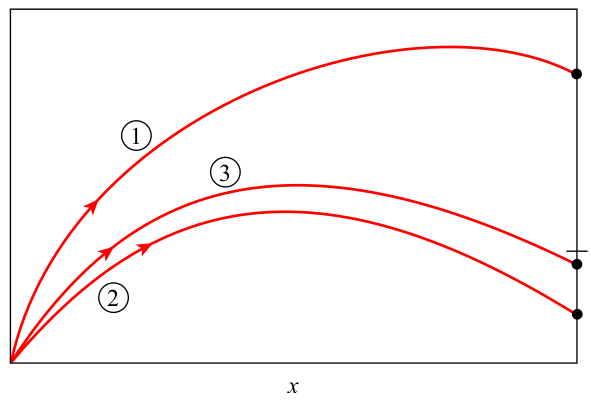
\includegraphics[width = 110mm]{ODE_konspect.png}}
        \caption{Метод стрельбы, надо попасть как можно ближе к горизонтальной черточке на правом конце. Первый раз промахнулись, прикинули как изменить параметры траектории, чтобы попасть ближе к чёрточке и т.д.}
        \label{graph1}
    \end{figure} 
\subsubsection{Двумерный случай}
    Проиллюстрируем применение метода стрельбы на уравнении 2--го порядка (то есть две неизвестных функции от $x$ и два уравнения)
    \begin{equation}
    \begin{cases}
        u'(x) = f(x, u,v)\\ v'(x)=g(x,u,v)
    \end{cases}
    x \in [a,\ b]
    \end{equation}
    с условием $$\phi (u(a),v(a)) = 0, \quad \psi(u(b),v(b))=0.$$
    \par
    Тогда из точки $x=a$ можем выпускать целую серию траекторий. Возьмём, например, $u(a)=\eta,\ v(a)=\zeta(\eta)$. Подставляем в условие на левом конце и находим $\zeta(\eta)$. Таким образом начальная точка определяется только одним параметром~---~параметром $\eta$. Тогда, решая уравнение, получаем параметрически заданное семейство траекторий $u(x,\eta),\ v(x,\eta)$. Теперь можно получить уравнение на $\eta$, подставив $u(x,\eta),\ v(x,\eta)$ в условие на правом конце: $$\Psi(\eta) = \psi(u(x,\eta),\ v(x,\eta)) = 0.$$ Далее получаем линейное уравнение и находим желанное $\eta$ из него.
    \par
    Трудности возникают только при сложных функциях $f(x, u,v)$ и $g(x,u,v)$, ведь в таком случае они решаются с конечной точностью, значит, уравнение $\Psi(\eta) = 0$ решается с огромными ошибками, что делает метод малоприменимым.
\subsubsection{Многомерный случай}
    Элементарное обобщение на многомерный случай. Пускай у нас есть $p$ уравнений
    \begin{equation}
     u_k'(x) = f_k(x, \boldsymbol u),\ \ \ k=1, \ldots,p,\ \ \ x \in [a,\ b]
    \end{equation}
    с граничными условиями
    \begin{equation}\label{***}
     \phi_i (\boldsymbol u(a)) = 0,\ \ \ i=1, \ldots,m \ge p/2,
    \end{equation}
    \begin{equation}\label{***+}
     \psi_j (\boldsymbol u(b)) = 0,\ \ \ j=1, \ldots,p-m.
    \end{equation}
    Заметим, что $m \ge p/2$ требуется не просто так, а по причине того, что в противном случае, уравнение в точке $b$ может стать слишком сложным, слишком много будет в нём переменных, при том что точность и так низкая (как уже говорилось выше), получим очень плохо численно решаемое уравнение.\par
    Так вот, опять строим $\boldsymbol u(a)=\boldsymbol \eta$~---~запускаем семейство лучей из $a$. Подставляем в (\ref{***}), остаётся $p-m$ независимых $\eta$. Тогда запускаем траектории, считаем значение функции в точки $b$, подставляем её в (\ref{***+}) и получаем $p-m$ уравнений на $p-m$ независимых $\eta$.
    \begin{equation}
     \boldsymbol \Psi_j(\eta_1,\ldots, \eta_{p-m})= \psi_j (\boldsymbol u(b, \boldsymbol \eta)) = 0.
    \end{equation}
    \par
    Основная проблема этих уравнений на $\boldsymbol \eta$ в том, что мы очень плохо знаем $\boldsymbol u$. Она вычисляется в сложных случаях долго с большой погрешностью. Поэтому метод стрельбы используют только в случаях малого $p-m$.
\subsection{Разностный метод (Relaxation)}
    Для более сложных систем используют не метод стрельбы, а разностный метод. В чём его идея? {У нас есть отрезок, строим на нём сетку, получаем дискретную функцию, аппроксимируем её производные конечными разностями, таким образом вместо системы ОДУ получаем систему линейных алгебраических уравнений на $\boldsymbol u$. Теперь эту систему можно решать, тут на помощь приходит интерполяционный метод.}\par
    Рассмотрим опять уравнение второго порядка. Будем иметь дело с таким уравнением с данными граничными условиями:
    \begin{equation}
     u'(x) = f(x, u),\ \ \ u(a)=\alpha,\ \ \ u(b) = \beta, \ \ \ x \in [a,\ b].
    \end{equation}
    Идея состоит в том, что мы аппроксимируем по симметричным точкам вторую производную, получаем такую вещь:
    \begin{equation}\label{48}
     u_{n+1} - 2 u_n + u_{k-1} = h^2f(x_n, u_n) + O(h^4).
    \end{equation}
    Берём значение $g(x, u)$ в средней точке и получаем погрешность четвёртого порядка.\par
    Но что такое мы получили? Мы получили в (\ref{48}) уравнение на вектора $\boldsymbol u$ с трёхдиагональной матрицей. И проблема в том, что это уравнение не линейное. Будь оно линейным, мы бы взяли да и перенесли правую часть влево, обернули трёхдиагональную матрицу и всё было бы хорошо, а так нет.\par
    Приходится решать такое уравнение итерациями:
    \begin{equation}
     u_{n+1}^{(s)} - 2 u_n^{(s)} + u_{k-1}^{(s)} = h^2f(x_n, u_n^{(s-1)}),
    \end{equation}
    с граничными условиями$$u_1^{(s)}=\alpha,\ u_N^{(s)} = \beta.$$
    Оказывается, что метод сходится со скоростью равной $2$. То есть он квадратичный по итерациям. Если узлов сетки очень много, хотя бы сотни или тысячи, то решать линейную систему очень не приятно.\par
    Данный метод с помощью введения дополнительной симметризации обобщается на многомерье. То есть задаём правую часть симметричным образом:
    \begin{equation}
     \boldsymbol u_k - \boldsymbol u_{k-1} = h \boldsymbol f(\frac{x_k + x_{k-1}}{2}, \frac{\boldsymbol u_k + \boldsymbol u_{k-1}}2).
    \end{equation}
    Это понизит погрешность, ошибка будет $\sim h^2$, что уже не плохо. Однако становится больше нетривиальных элементов матрицы и свой вклад в это вносят и граничные условия:
    \begin{equation}
     \varphi_i (x_1,\boldsymbol u_1) = 0,\ \ \ \psi_j (x_N,\boldsymbol u_N) = 0.
    \end{equation}
    Это, конечно, делает задачу более сложной, но вполне решаемой итерационным методом.
\subsection{Метод Галеркина}
    Решать для большого числа точек алгебраическую систему~---~не самая простая вещь, так как в одномерном случае трёхдиагональную матрицу ещё легко обернуть прогонкой, а вот в общем случаем, матрица становится сложнее и оборачивать её уже долго.\par
    В таком случае обычно применяют метод Галеркина. {Это метод разложения по полной системе функций.}\par
    Пускай у нас $\varphi_k (x)$~---~полная система функций такая, что функции обращаются в нуль на краях интервала $\varphi_k (a) =\varphi_k (b) = 0$. И метод Галеркина основан на том, что если для какой-то $F(x)$
    \begin{equation}
     \forall \quad k\ge1: \quad\int_a^b F(x)\varphi_k (x)dx=0 \Rightarrow F(x) \equiv 0.
    \end{equation}
    То есть функция $F(x)$ тождественный нуль. Справедливо и обратное утверждение. Как это работает для краевой задачи?\par
    Пусть написали разностную схему $\hat A [u(x)]=f(x)$ с заданными краевыми условиями $u(a)=\alpha,\  u(b) = \beta, \ x \in [a,\ b]$. Тогда решение удобней искать по полной системе функций
    \begin{equation}\label{53}
     u(x) \approx \varphi_0(x) + \sum_{k=1}^nc_k\varphi_k(x),
    \end{equation}
    где функция $\varphi_0(x)$ равна альфа и бета на границе, а все остальные на границе обращаются в нуль 
    \begin{equation}
     \varphi_k(a)=\alpha\delta_{k,0},\ \ \varphi_k(b)=\beta\delta_{k,0}.
    \end{equation}
    Тогда рассматриваем такой интеграл и подставляем в него $u(x)$ из (\ref{53}), чтобы затем получить систему уравнений на $c_k$.
    \begin{equation}
     \int_a^b \biggl(\hat A [u(x)] - f(x)\biggr)\varphi_k(x)dx = 0,\ \ \ k=1,\ldots,n.
    \end{equation}\par
    Единственная проблема в том, что если бы уравнение было бы линейное по $c_k$, то эта задача сразу бы решалась обращением матрицы, а коли она у нас не линейная, то приходится опять решать систему алгебраических уравнений методом итераций. Приходится брать $n$ не очень большим, но задача в принципе решается, то есть удаётся получить аппроксимацию по полной системе функций со вполне разумной точностью. Это приближение можно использовать, как начальное условие для разностного метода, например.
\subsection{Разрывные коэффициенты}
    Вопрос: что делать, коли внутри нашего интервала образовались разрывные коэффициенты (то есть {функция или/и её производная терпят разрыв, резкий скачок где-то на интервале})? Примером такой ситуации может служить столбик водичка--маслецо, ведь когда пытаемся просчитать распространение, например, светового пучка сквозь такую среду, коэффициент преломления сильно скачет на границе двух жидкостей.\par
    {В данном случае} обычная аппроксимация уже не спасёт. {Нужно писать правильным образом граничные условия на разрыве}. Обычно это непрерывность функции искомой $\boldsymbol u(x)$, её производной $\boldsymbol u'(x)$ или {в общем случае какая-то их комбинация, типа $\alpha \boldsymbol u(x_* - 0) + \beta \boldsymbol u'(x_* - 0) =\alpha \boldsymbol u(x_* + 0) + \beta \boldsymbol u'(x_* + 0)$.}\par
    Таким образом приходится вводить новое граничное условие на сетке (если решаем сеточными методами). Это часто приводит к потере единственности решения, что для численного метода ужасно плохо. Если же методом Галеркина решаем задачу, то следует выбирать функции $\varphi_k(x)$ так, чтобы они удовлетворяли новому граничному условию.
    
    \begin{thebibliography}{1}
     \bibitem{wiki_l}
     Николай Николаевич Лузин. Дифференциальное исчисление / С.И. Новосёлова. — 1-е. — Москва, Б-62, Подсосенский пер. 20: Государственное издательство ''Высшая Школа'' , 1961. — С. 326. — 477 с.
     \bibitem{tkv}
     Курс лекций ''Теория колебаний и волн'', автор: Алексей Антониевич Балакин. Лекции доступны по ссылке:\\
     \url{https://enabla.com/ru/set/12/pub/223}
    \end{thebibliography}

\end{document}
